\newpage 
\section{Theoretical framework}

\subsection{Plasma and Magnetic Confinement Fundamentals}

\subsubsection{Basic Plasma Parameters and the Confinement Criterion}
A common definition of plasma is that it is a quasineutral ionized gas that exhibits collective behavior, requiring the physical system dimensions $L$ to be greater than the Debye length $\lambda_D$ ($\text{m}$) \cite{chen2016introduction}, defined in equation \ref{eqn:debye}:
\begin{equation}
\label{eqn:debye}
    \lambda_D = \sqrt{\frac{\varepsilon_0 k_B T_e}{n_e e^2}}
\end{equation}
Where $\varepsilon_0$ is the vacuum permittivity ($\text{F/m}$), $k_B$ is the Boltzmann constant ($\text{J/K}$), $T_e$ is the electron temperature ($\text{K}$), $n_e$ is the electron density ($\text{m}^{-3}$), and $e$ is the fundamental charge ($\text{C}$). Quasineutrality, defined in equation \ref{eqn:quasi}, applies macroscopically but fails within $\lambda_D$, where strong electric fields persist \cite{chen2016introduction}:
\begin{equation}
    \label{eqn:quasi}
    n_i \simeq n_e \simeq n
\end{equation}
Where $n_i$ is the ion density ($\text{m}^{-3}$) and $n$ is the plasma density ($\text{m}^{-3}$). Collective plasma behavior is characterized by the electron plasma frequency $\omega_{pe}$ ($\text{Hz}$), expressed in equation \ref{eqn:plasmafreq} \cite{chen2016introduction}:
\begin{equation}
    \label{eqn:plasmafreq}
    \omega_{pe} = \sqrt{\frac{n_e e^2}{m_e \varepsilon_0}}
\end{equation}
Where $m_e$ is the mass of the electron ($\text{kg}$). In order to obtain a positive fusion energy production, the confinement parameters must satisfy the Lawson criterion given in equation \ref{eqn:Lawson}, ensuring the fusion reaction liberates more energy than required to sustain it \cite{chen2016introduction}:
\begin{equation}
\label{eqn:Lawson}
n \tau_E T \ge 3 \times 10^{21} \text{ m}^{-3}\ \text{s}\ \text{keV}
\end{equation}
Where $\tau_E$ is the energy confinement time ($\text{s}$) and $T$ is the plasma temperature ($\text{keV}$). The plasma $\beta$ parameter measures the ratio of kinetic pressure to magnetic pressure, and it is defined in equation \ref{eqn:beta} \cite{chen2016introduction}:
\begin{equation} 
\label{eqn:beta}
\beta = \frac{\sum_j n_j k_B T_j}{\frac{B^2}{2\mu_0}}
\end{equation}
Where $j$ is the species index, $n_j$ is the number density of species $j$ ($\text{m}^{-3}$), $T_j$ is the temperature of species $j$ ($\text{K}$), $B$ is the magnetic field ($\text{T}$), and $\mu_0$ is the vacuum permeability ($\text{H/m}$).

\subsubsection{MHD Equations and Equilibrium}
The ideal MHD equations describe macroscopic plasma behavior, coupling fluid dynamics to Maxwell's equations through momentum, Ohm's law, state, mass continuity, Amp\`ere's, and Faraday's laws, presented in equations \ref{eqn:MHD_momentum} to \ref{eqn:MHD_Faraday}, respectively \cite{zheng, chen2016introduction}:
\begin{align} 
\rho \frac{d\mathbf{u}}{dt} &= -\nabla P + \mathbf{J} \times \mathbf{B}, \label{eqn:MHD_momentum} \\ 
\mathbf{E} &= -\mathbf{u} \times \mathbf{B}, \label{eqn:MHD_Ohm} \\ 
\frac{\partial P}{\partial t} &= -\mathbf{u} \cdot \nabla P - \Gamma P \nabla \cdot \mathbf{u}, \label{eqn:MHD_State} \\ 
\frac{\partial \rho}{\partial t} &= -\mathbf{u} \cdot \nabla \rho - \rho \nabla \cdot \mathbf{u}, \label{eqn:MHD_mass_continuity} \\ 
\mu_0 \mathbf{J} &= \nabla \times \mathbf{B}, \label{eqn:MHD_Ampere} \\ 
\frac{\partial \mathbf{B}}{\partial t} &= -\nabla \times \mathbf{E}, \label{eqn:MHD_Faraday} 
\end{align}
Where $\rho$ is the mass density ($\text{kg/m}^3$), $\mathbf{u}$ is the fluid velocity vector ($\text{m/s}$), $t$ is the time ($\text{s}$), $P$ is the thermal pressure ($\text{Pa}$), $\mathbf{J}$ is the current density vector ($\text{A/m}^2$), $\mathbf{B}$ is the magnetic field vector ($\text{T}$), $\mathbf{E}$ is the electric field vector ($\text{V/m}$), and $\Gamma$ is the adiabatic index. Static MHD equilibrium dictates that nested magnetic flux surfaces support the plasma pressure gradient, formulated in equation \ref{eqn:MHD_equilibrium}:
\begin{equation}
\label{eqn:MHD_equilibrium}
\mathbf{J} \times \mathbf{B} = \nabla p 
\end{equation}
Where $p$ is the kinetic plasma pressure ($\text{Pa}$). Perturbations to this equilibrium excite shear Alfv\'en waves propagating along magnetic flux surfaces \cite{zheng, chen2016introduction}.

\subsection{The Heliotron J Device}
Heliotron J is a helical-axis heliotron generated by an $L=1, M=4$ continuous helical coil, employing varied toroidal and vertical field coils to produce a rotational transform without a net toroidal current \cite{chen2016introduction, Miyazawa2023, Yamamoto_2020}. Heating relies on Neutral Beam Injection (NBI), providing non-Maxwellian energetic ions that serve as the primary drive for kinetic MHD modes, and 70 GHz Electron Cyclotron Heating (ECH) for localized resonance \cite{nagasaki2020heliotron}. Diagnostics utilized include: toroidal and poloidal Mirnov coil arrays (MP1--MP4 and PMP1--PMP14) for magnetic fluctuations; diamagnetic loops measuring macroscopic stored energy $W_p$; Electron Cyclotron Emission (ECE) for electron temperature profiles; and Langmuir/H$_\alpha$FAST arrays for edge characterization \cite{nagasaki2020heliotron}. This heating and diagnostic systems locations on the Heliotron J can be observed in the figure \ref{fig:locations}.

\begin{figure}[H]
  \centering
  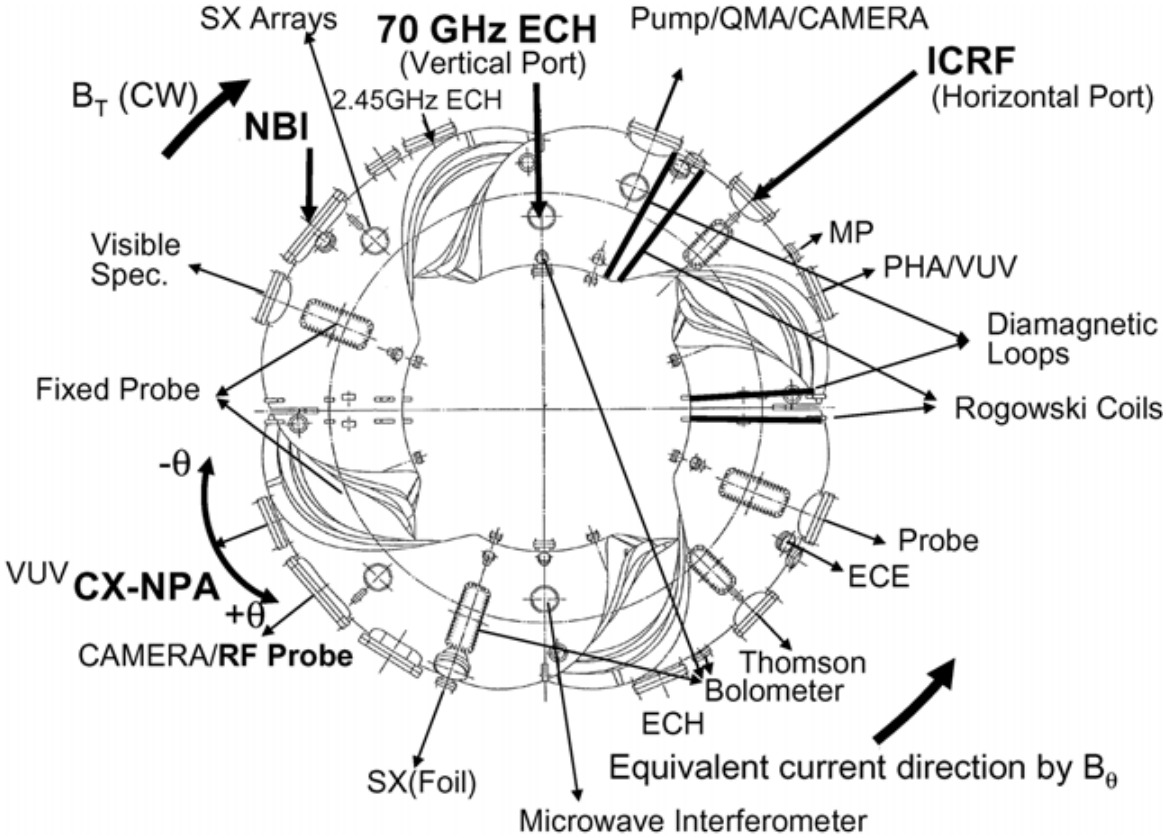
\includegraphics[width=0.7\textwidth]{Images/Locations.jpeg}
  \caption[Heating and diagnostic systems in Heliotron J]{Heating and diagnostic systems in Heliotron J \cite{Okada2007}.}
  \label{fig:locations}
\end{figure}



\subsection{MHD Instabilities and Alfv\'en Eigenmodes}

\subsubsection{Energetic-Particle-Driven Modes}
Energetic particles (EPs) injected by NBI exhibit a bump-on-tail velocity distribution, providing free energy to resonantly destabilize background modes \cite{Sheikh2023, Adulsiriswad_2024, Varela2015}. Shear Alfv\'en waves propagate at the Alfv\'en velocity $v_A$ ($\text{m/s}$), defined in equation \ref{eqn:alfven} \cite{chen2016introduction}:
\begin{equation}
\label{eqn:alfven}
v_A = \frac{B}{\sqrt{\mu_0 n_i m_i}}
\end{equation}
Where $m_i$ is the ion mass ($\text{kg}$). In 3D helical systems, non-axisymmetric geometric couplings open discrete frequency gaps allowing Alfv\'en eigenmodes (AEs) to exist without heavy continuum damping \cite{Varela2015, Adulsiriswad_2024}. Instability requires the wave--particle resonance defined in equation \ref{eqn:condition} \cite{Adulsiriswad_2024}:
\begin{equation}
\label{eqn:condition}
\omega - n\omega_\phi + L\omega_\theta = 0
\end{equation}
Where $\omega$ is the mode angular frequency ($\text{rad/s}$), $n$ is the toroidal mode number, $\omega_\phi$ is the energetic particle toroidal transit frequency ($\text{rad/s}$), $L$ is the integer harmonic, and $\omega_\theta$ is the energetic particle poloidal drift frequency ($\text{rad/s}$). Mode spatial periodicity is defined in equation \ref{eqn:periodicity}:
\begin{equation}
\label{eqn:periodicity}    
\exp\left[i(m\theta - n\zeta)\right]
\end{equation}
Where $m$ is the poloidal mode number, $\theta$ is the poloidal coordinate ($\text{rad}$), and $\zeta$ is the toroidal coordinate ($\text{rad}$). Resonance occurs at the rational flux surface defined in equation \ref{eqn:varela} \cite{Varela2015}:
\begin{equation}
\label{eqn:varela}
    \iota/2\pi = n/m
\end{equation}
Where $\iota$ is the rotational transform ($\text{rad}$).

\subsubsection{Theoretical Frequency Scaling Models}
To physically classify instabilities, instantaneous frequencies are compared against established scaling models \cite{Varela2024}. Shear Alfv\'en scaling is defined in equation \ref{eqn:shear_alfven}:
\begin{equation}
\label{eqn:shear_alfven}
f_A(t) \propto \frac{v_A(t)}{q R_0} \propto \frac{B}{\sqrt{n_e(t)}}
\end{equation}
Where $f_A(t)$ is the instantaneous shear Alfv\'en frequency ($\text{Hz}$), $q$ is the safety factor, and $R_0$ is the major radius ($\text{m}$). Beta-induced Alfv\'en Eigenmodes (BAE) and Geodesic Acoustic Modes (GAM) scale with temperature as shown in equation \ref{eqn:gam}:
\begin{equation}
\label{eqn:gam}
f_{\text{BAE}}(t) \propto \sqrt{T_e(t)}
\end{equation}
Where $f_{\text{BAE}}(t)$ is the instantaneous Beta-induced Alfv\'en Eigenmode frequency ($\text{Hz}$). Compressibility coupled scaling is given by equation \ref{eqn:compressibility}:
\begin{equation}
\label{eqn:compressibility}
f(t) \propto \sqrt{\frac{C_1}{n_e(t)} + C_2 T_e(t)}
\end{equation}
Where $f(t)$ is the compressibility-coupled mode frequency ($\text{Hz}$), and $C_1$ and $C_2$ are scaling constants. Beam-driven Energetic Particle Modes (EPMs) scale via density gradients or drift resonance, presented in equations \ref{eqn:epm_density} and \ref{eqn:epm_drift}:
\begin{equation}
\label{eqn:epm_density}
f_{\text{EPM}}(t) \propto \sqrt{\frac{P_{\text{NBI}}(t)}{n_e(t)}}
\end{equation}
\begin{equation}
\label{eqn:epm_drift}
f_{\text{EPM}}(t) \propto P_{\text{NBI}}(t)
\end{equation}
Where $f_{\text{EPM}}(t)$ is the Energetic Particle Mode frequency ($\text{Hz}$) and $P_{\text{NBI}}(t)$ is the Neutral Beam Injection heating power ($\text{W}$). Macroscopic mode shifts due to plasma current and finite-$\beta$ energy are modeled by equation \ref{eqn:shift_macro}:
\begin{equation}
\label{eqn:shift_macro}
f(t) \propto I_p(t), \quad f(t) \propto W_p(t)
\end{equation}
Where $I_p(t)$ is the plasma current ($\text{A}$) and $W_p(t)$ is the macroscopic stored energy ($\text{J}$).

\subsection{Signal Processing for MHD Mode Characterization}

\subsubsection{Time-Frequency Analysis}
Spectral resolution $\Delta f$ ($\text{Hz}$) for standard Fast Fourier Transform (FFT) windows is defined in equation \ref{eqn:freq_res} \cite{proakis2021digital}:
\begin{equation}
\label{eqn:freq_res}
\Delta f = \frac{1}{T}
\end{equation}
Where $T$ is the window duration ($\text{s}$). For non-stationary events, Fourier analysis fails to capture rapid transitions \cite{boashash2015time}. This is why, the Continuous Wavelet Transform, which uses the Morlet wavelet, is chosen, due to its fine temporal resolution at high frequencies, defined in equation \ref{eqn:morlet} \cite{addison2016illustrated}:
\begin{equation}
\label{eqn:morlet}
\psi(t) = \pi^{-1/4} e^{i \omega_0 t} e^{-\frac{t^2}{2}}
\end{equation}
Where $\psi(t)$ is the Morlet wavelet function  and $\omega_0$ is the central frequency parameter ($\text{rad/s}$). Dominant modes must exceed a $3\sigma$ noise baseline calculated over a quiescent pre-plasma phase, defined in equation \ref{eqn:dominance} \cite{Edlund2018}, and exhibit global spatial coherence to distinguish modes from single-channel noise \cite{KraemerFlecken2024, Singh2024}, defined in equation \ref{eqn:coherence}:
\begin{equation}
\label{eqn:dominance}
P(f, t) \ge \mu_{\text{noise}}(f) + 3\sigma_{\text{noise}}(f)
\end{equation}
Where $P(f, t)$ is the power spectral density ($\text{V}^2/\text{Hz}$), $f$ is the frequency ($\text{Hz}$), $\mu_{\text{noise}}(f)$ is the spectral mean of the noise baseline ($\text{V}^2/\text{Hz}$), and $\sigma_{\text{noise}}(f)$ is the standard deviation of the noise baseline ($\text{V}^2/\text{Hz}$).
\begin{equation}
\label{eqn:coherence}
\gamma_{xy}^2(f) = \frac{|P_{xy}(f)|^2}{P_{xx}(f) P_{yy}(f)}
\end{equation}
Where $\gamma_{xy}^2(f)$ is the magnitude-squared spatial coherence, $P_{xy}(f)$ is the cross-spectral density ($\text{V}^2/\text{Hz}$), and $P_{xx}(f)$ and $P_{yy}(f)$ are the auto-spectral densities ($\text{V}^2/\text{Hz}$).

\subsubsection{Toroidal Mode Identification \& Radial Localization}
Toroidal mode number is obtained via cross-spectral phase at frequency $f_0$, defined in equation \ref{eqn:meas_phase}\cite{bendat2010random,Smith1971}:
\begin{equation}
\label{eqn:meas_phase}
\Delta\phi_{ij}^{\text{meas}} = \arg\left[P_{x_i x_j}(f_0)\right]
\end{equation}
Where $\Delta\phi_{ij}^{\text{meas}}$ is the measured cross-spectral phase ($\text{rad}$), $f_0$ is the peak mode frequency ($\text{Hz}$), and $x_i$ and $x_j$ are the respective probe signals ($\text{V}$). The theoretical spatial phase shift is given by equation \ref{eqn:theo_phase} \cite{strait2006,Seo2019TheEO}:
\begin{equation}
\label{eqn:theo_phase}
\Delta\phi_{ij}^{\text{theo}}(n) = (n \Delta\varphi_{ij} + \pi) \pmod{2\pi} - \pi
\end{equation}
Where $\Delta\phi_{ij}^{\text{theo}}(n)$ is the theoretical spatial phase shift ($\text{rad}$) and $\Delta\varphi_{ij}$ is the geometric toroidal separation angle ($\text{rad}$). The best-fit $n$ minimizes the root mean square (RMS) phase error, defined in equation \ref{eqn:rmse}, incorporating coplanar selection rules to avoid spatial aliasing\cite{schittenhelm1997analysis}:
\begin{equation}
\label{eqn:rmse}
\text{RMSE}(n) = \sqrt{\frac{1}{N_{\text{pairs}}} \sum_{(i,j)} \left(\Delta\phi_{ij}^{\text{meas}} - \Delta\phi_{ij}^{\text{theo}}(n)\right)^2}
\end{equation}
Where $\text{RMSE}(n)$ is the RMS error ($\text{rad}$) and $N_{\text{pairs}}$ is the number of evaluated probe pairs. Radial localization utilizes ECE radial temperature fluctuation profiles, extracted as shown in equation \ref{eqn:ece_rms}, mapping the perturbation peak via cross-coherence with Mirnov signals \cite{luo2020measurement}:
\begin{equation}
\label{eqn:ece_rms}
\tilde{T}_e(r) = \text{std}(\text{filt}(y_{\text{ECE}}))
\end{equation}
Where $\tilde{T}_e(r)$ is the RMS electron temperature fluctuation ($\text{K}$), $r$ is the radial coordinate ($\text{m}$), and $y_{\text{ECE}}$ is the raw Electron Cyclotron Emission signal ($\text{V}$).

\subsection{Signal Conditioning and Correlation Analysis}

\subsubsection{Instantaneous Parameters \& Envelope Dynamics}
Magnetic signals are conditioned using a Bessel bandpass filter, selected for its maximally flat group delay to prevent phase distortion \cite{zang2019observation}. The analytic signal is constructed via the Hilbert transform to extract unwrapped phase and instantaneous amplitude \cite{Fabus2021}. Prior to correlation, data also undergoes low-pass filtering and anti-aliasing decimation to strictly respect the temporal Nyquist limit \cite{Fabus2021, boashash2015time}. 

Wave-packet beating creates envelope modulation, defined in equation \ref{eqn:f_mod}:
\begin{equation}
\label{eqn:f_mod}
f_{\text{mod}} = f_0 - f_1
\end{equation}
Where $f_{\text{mod}}$ is the envelope modulation frequency ($\text{Hz}$) and $f_1$ is the lower carrier frequency ($\text{Hz}$). Carrier-envelope self-coupling coherence is evaluated via equation \ref{eqn:self_coupling} \cite{bendat2010random}:
\begin{equation}
\label{eqn:self_coupling}
\gamma_{\tilde{B}, A}^2(f) = \frac{|P_{\tilde{B} A}(f)|^2}{P_{\tilde{B}\tilde{B}}(f) P_{AA}(f)}
\end{equation}
Where $\gamma_{\tilde{B}, A}^2(f)$ is the self-coupling coherence , $P_{\tilde{B} A}(f)$ is the cross-spectral density between the carrier and envelope ($\text{V}^2/\text{Hz}$), $P_{\tilde{B}\tilde{B}}(f)$ is the carrier auto-spectral density ($\text{V}^2/\text{Hz}$), and $P_{AA}(f)$ is the envelope auto-spectral density ($\text{V}^2/\text{Hz}$). This must exceed the statistical noise floor formulated in equation \ref{eqn:noise_floor} \cite{carter1973estimation}:
\begin{equation}
\label{eqn:noise_floor}
\gamma_{95}^2 = 1 - (0.05)^{1/(N_{\text{seg}} - 1)}
\end{equation}
Where $\gamma_{95}^2$ is the 95 percent statistical noise floor and $N_{\text{seg}}$ is the number of averaging segments.

\subsubsection{Spatial Harmonic Decomposition \& Poloidal Phase}
To resolve the poloidal structure across non-uniform probes and prevent spatial aliasing \cite{Varela2019}, the spatial non-uniform discrete Fourier transform (NUDFT) is computed via equation \ref{eqn:nudft} \cite{dutt1993fast}:
\begin{equation}
\label{eqn:nudft}
S_k = \frac{1}{N_{\text{probes}}} \sum_{j=1}^{N_{\text{probes}}} S_j e^{-i k \theta_j}
\end{equation}
Where $S_k$ is the spatial spectral component at wavenumber $k$ ($\text{V}$), $k$ is the discrete poloidal wavenumber, $N_{\text{probes}}$ is the total number of probes, $S_j$ is the complex spectral component of probe $j$ ($\text{V}$), and $\theta_j$ is the poloidal angle of probe $j$ ($\text{rad}$). Cross-spectral poloidal phase relative to a reference probe is extracted using equation \ref{eqn:pol_phase} \cite{Smith1971}:
\begin{equation}
\label{eqn:pol_phase}
\phi_j = \arg\left[\langle S_j(f) S_{\text{ref}}^*(f) \rangle\right] - \phi_{\text{ref}}
\end{equation}
Where $\phi_j$ is the cross-spectral poloidal phase of probe $j$ ($\text{rad}$), $S_{\text{ref}}$ is the complex spectral component of the reference probe ($\text{V}$), and $\phi_{\text{ref}}$ is the phase of the reference probe ($\text{rad}$). This is subject to the Bendat-Piersol metrological phase uncertainty established in equation \ref{eqn:phase_uncert} \cite{bendat2010random}:
\begin{equation}
\label{eqn:phase_uncert}
\sigma_{\phi, j} = \sqrt{\frac{1 - \gamma_j^2}{2 \gamma_j^2 N_{\text{seg}}}}
\end{equation}
Where $\sigma_{\phi, j}$ is the metrological phase uncertainty ($\text{rad}$) and $\gamma_j^2$ is the coherence of probe $j$ with the reference probe. A phase good fit is verified by the Mardia-Jupp circular correlation coefficient, calculated via equation \ref{eqn:r_circ} \cite{mardia2000directional}:
\begin{equation}
\label{eqn:r_circ}
r_{\text{circ}}(m) = \frac{1}{N} \sqrt{\left(\sum \cos(\phi_j - m\theta_j)\right)^2 + \left(\sum \sin(\phi_j - m\theta_j)\right)^2}
\end{equation}
Where $r_{\text{circ}}(m)$ is the circular correlation coefficient and $N$ is the sample size of probes. Valid poloidal structures strictly require $r_{\text{circ}} \ge 0.70$ and a mean absolute phase error $\overline{|\Delta\phi|} \le 45^\circ$, evaluated after correcting known hardware polarity inversions.

\subsubsection{Correlation and Significance}
Lagged cross-correlation identifies dynamic heating response delays \cite{Zhong2020}, defined in equation \ref{eqn:lagged_corr}:
\begin{equation}
\label{eqn:lagged_corr}
R_{xy}(\tau) = \frac{1}{N} \sum_{t} \left(\frac{x(t) - \bar{x}}{\sigma_x}\right)\left(\frac{y(t+\tau) - \bar{y}}{\sigma_y}\right)
\end{equation}
Where $R_{xy}(\tau)$ is the lagged cross-correlation, $\tau$ is the time lag ($\text{s}$), $x(t)$ and $y(t)$ are the time-series signals ($\text{V}$), $\bar{x}$ and $\bar{y}$ are their respective sample means ($\text{V}$), and $\sigma_x$ and $\sigma_y$ are their sample standard deviations ($\text{V}$). These empirical delays are physically motivated by the fast-ion slowing-down timescale defined in equation \ref{eqn:slowing_down} \cite{Salewski2025}:
\begin{equation}
\label{eqn:slowing_down}
\tau_s \approx 6.27 \times 10^8 \frac{A_b T_e^{3/2}}{Z_b^2 n_e \ln \Lambda}
\end{equation}
Where $\tau_s$ is the slowing-down timescale ($\text{s}$), $A_b$ is the beam ion mass number, $Z_b$ is the beam ion charge number, and $\ln \Lambda$ is the Coulomb logarithm  \cite{chen2016introduction}, for this specific empirical constant, $T_e$ is strictly evaluated in $\text{eV}$, as it is common in plasma physics and $n_e$ in $\text{cm}^{-3}$. Effective sample size is constrained by autocorrelation using equation \ref{eqn:neff} \cite{shumway2017time}:
\begin{equation}
\label{eqn:neff}
N_{\text{eff}} = \frac{N}{1 + 2 \sum_{k=1}^{M} \rho(k)}
\end{equation}
Where $N_{\text{eff}}$ is the effective sample size, $M$ is the maximum evaluated lag, and $\rho(k)$ is the sample autocorrelation at lag $k$. Significance testing utilizes the $t$-statistic in equation \ref{eqn:t_stat} \cite{shumway2017time} and partial correlation in equation \ref{eqn:partial_corr} to isolate physical coupling from operational artifacts, evaluated alongside False Discovery Rate corrections \cite{james2021statistical}:
\begin{equation}
\label{eqn:t_stat}
t = r \sqrt{\frac{N_{\text{eff}} - 2 - n_{\text{control}}}{1 - r^2}}
\end{equation}
Where $t$ is the $t$-statistic, $r$ is the Pearson correlation coefficient, and $n_{\text{control}}$ is the number of control variables.
\begin{equation}
\label{eqn:partial_corr}
r_{xy \cdot z} = \frac{r_{xy} - r_{xz}r_{yz}}{\sqrt{(1 - r_{xz}^2)(1 - r_{yz}^2)}}
\end{equation}
Where $r_{xy \cdot z}$ is the partial correlation coefficient between $x$ and $y$ controlling for $z$, and $r_{xy}$, $r_{xz}$, and $r_{yz}$ are the respective pairwise Pearson correlation coefficients.

\subsection{Higher-Order Spectral Analysis for Nonlinear Wave Coupling}

\subsubsection{Bicoherence \& Coupling Domains}
Quadratic nonlinear three-wave coupling is detected via the auto-bispectrum defined in equation \ref{eqn:bispectrum}, measuring interactions that satisfy resonance matching \cite{proakis2021digital, Hou2019, Fujisawa2021}:
\begin{equation}
\label{eqn:bispectrum}
B(f_1, f_2) = \langle X(f_1) X(f_2) X^*(f_1 \pm f_2) \rangle
\end{equation}
Where $B(f_1, f_2)$ is the auto-bispectrum ($\text{V}^3/\text{Hz}^2$), $f_1$ and $f_2$ are the interacting frequencies ($\text{Hz}$), and $X(f)$ is the Fourier transform of the signal ($\text{V}/\text{Hz}$). Normalized phase-locking is quantified by the squared auto-bicoherence in equation \ref{eqn:bicoherence} \cite{Hou2019, proakis2021digital}:
\begin{equation}
\label{eqn:bicoherence}
b^2(f_1, f_2) = \frac{|\langle X(f_1) X(f_2) X^*(f_1 \pm f_2) \rangle|^2}{\langle |X(f_1) X(f_2)|^2 \rangle \langle |X(f_1 \pm f_2)|^2 \rangle}
\end{equation}
Where $b^2(f_1, f_2)$ is the squared auto-bicoherence. Significant coupling (typically $b^2 > 0.5$ \cite{Singh2024}) must exceed the statistical noise threshold formulated in equation \ref{eqn:b2_stat} to reject spurious background noise \cite{Hou2019, Fujisawa2021}:
\begin{equation}
\label{eqn:b2_stat}
b^2_\alpha = -\frac{\ln(\alpha)}{N_{\text{ensemble}}}
\end{equation}
Where $b^2_\alpha$ is the statistical significance threshold, $\alpha$ is the significance level, and $N_{\text{ensemble}}$ is the number of independent ensembles. To prevent redundant triad integration due to permutation symmetries, the spectra are mathematically partitioned into sum coupling (up-conversion) and difference coupling (parametric decay) regions, defined in equations \ref{eqn:sum_domain} and \ref{eqn:diff_domain}:
\begin{equation}
\label{eqn:sum_domain}
f_1 + f_2 = f_3 \quad (f_1 > 0, f_2 > 0)
\end{equation}
\begin{equation}
\label{eqn:diff_domain}
f_1 + f_2 = f_3 \quad (f_1 > 0, f_2 < 0)
\end{equation}
Where $f_3$ is the resultant coupled frequency ($\text{Hz}$).

\subsubsection{Bias Scaling \& Window Optimization}
Because finite-sample bicoherence exhibits an intrinsic positive bias ($\text{E}[\hat{b}^2] \approx 1/N$), physical triads are verified through the asymptotic scaling model shown in equation \ref{eqn:bias_extrap}, strictly requiring a non-zero intercept $b_\infty^2 > 0$ \cite{HinichWolinsky2005}:
\begin{equation}
\label{eqn:bias_extrap}
\hat{b}^2(N) = b_\infty^2 + \frac{C}{N}
\end{equation}
Where $\hat{b}^2(N)$ is the finite-sample squared bicoherence, $b_\infty^2$ is the asymptotic true bicoherence, and $C$ is a scaling constant. Coupled triads geometrically cluster along characteristic locations: subharmonic decay ($f_2 = -0.5f_1$), primary pump decay ($f_1 = f_{\text{pump}}$), and harmonic doubling ($f_1 = f_2$). Valid triads require adaptive temporal stationarity (minimizing instantaneous $|df/dt|$) and linear PSD peak correspondence ($\Delta f \le 1.5\text{ bins}$) \cite{HinichWolinsky2005}. 

\subsubsection{H-mode Burst-Window Detection and Validation}
To evaluate degraded transport, elevated coupling is cross-referenced against H-mode burst windows \cite{Kin2025, Miyashita2025}. A hysteresis algorithm triggers onset at $W_p \ge \mu_{\text{base}} + k_{\text{on}} \sigma_{\text{base}}$ and termination at $W_p \le \mu_{\text{base}} + k_{\text{off}} \sigma_{\text{base}}$. The statistical exclusivity of burst bicoherence is evaluated against the quiescent phase using a non-parametric Kruskal-Wallis test, visible on the equation \ref{eq:kruskal} \cite{shumway2017time, james2021statistical}. 

\begin{equation} \label{eq:kruskal}
H = \frac{12}{N(N+1)} \sum_{i=1}^{k} \frac{R_i^2}{n_i} - 3(N+1)
\end{equation}
Where $H$ is the Kruskal-Wallis test statistic, $N$ is the total number of observations across all groups, $k$ is the number of groups compared, $n_i$ is the number of observations in group $i$, and $R_i$ is the sum of ranks for group $i$.

This is followed by post-hoc Mann-Whitney U tests to identify specific pairwise differences, calculated via equation \ref{eq:mannwhitney}:
\begin{equation} \label{eq:mannwhitney}
U_1 = n_1 n_2 + \frac{n_1(n_1+1)}{2} - R_1
\end{equation}
Where $U_1$ is the Mann-Whitney U test statistic for group 1, $n_1$ and $n_2$ are the sample sizes for group 1 and group 2, and $R_1$ is the sum of the ranks for group 1.

To control the family-wise error rate across multiple comparisons, a Bonferroni correction is applied to the significance level, as shown in equation \ref{eq:bonferroni}:
\begin{equation} \label{eq:bonferroni}
\alpha_{adj} = \frac{\alpha}{m}
\end{equation}
Where $\alpha_{adj}$ is the adjusted significance level, $\alpha$ is the original target significance level, such as 0.05, and $m$ is the total number of independent hypotheses or pairwise comparisons evaluated.





Physical validation demands cross-diagnostic consistency, matching Mirnov triads to Langmuir electrostatic measurements ($\Delta f \le 10\text{ kHz}$) \cite{Kin2025}. Spatial false-positive rejection applies the effective number of independent channels, calculated in equation \ref{eqn:meff} \cite{Bishop2023, Afyouni2019}:
\begin{equation}
\label{eqn:meff}
M_{\text{eff}} = \sum_{i=1}^{N_{\text{tips}}} \min(\lambda_i, 1)
\end{equation}
Where $M_{\text{eff}}$ is the effective number of independent channels, $N_{\text{tips}}$ is the number of probe tips, and $\lambda_i$ is the $i$-th eigenvalue of the correlation matrix. Capping the family-wise spatial chance probability defined in equation \ref{eqn:p_chance}:
\begin{equation}
\label{eqn:p_chance}
P_{\text{chance}} = 1 - \left(1 - \frac{4 (\Delta f)^2}{f_{1,\max} f_{2,\max}}\right)^{M_{\text{eff}} \cdot N_{\text{MP}}}
\end{equation}
Where $P_{\text{chance}}$ is the family-wise spatial chance probability, $f_{1,\max}$ and $f_{2,\max}$ are the maximum search frequencies ($\text{Hz}$), and $N_{\text{MP}}$ is the number of evaluated Mirnov channels. Final confirmation establishes that elevated three-wave coupling coincides with a degraded rate of stored energy change ($dW_p/dt \le 0\text{ kJ/s}$), mediating enhanced turbulent transport \cite{Hou2019, Fujisawa2021}.